% TYPES OF PHYLOGENIES AND REPRESENTATIONS
\begin{frame}
\frametitle{Types of phylogenies and representations}

\begin{columns}

\column{0.66\textwidth}

\begin{centering}

rooted trees

\end{centering}

\column{0.34\textwidth}

\begin{centering}

unrooted tree

\end{centering}

\end{columns}

\begin{columns}[b]

\column{0.33\textwidth}

\begin{centering}

% Auto-generated from TikzTree.java
% xScale=-0.5 yScale=-0.5 offset=0.2
% scalebar=null
% options=[ultra thick]
% newick=((((A: 1, B: 1): 1, C: 2): 1, D: 3): 1, E: 4);
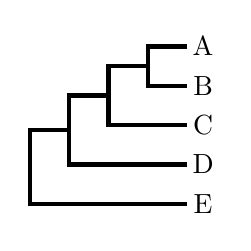
\begin{tikzpicture}[ultra thick]

\node at (0.2, 0.0) {A};
\node at (0.2, -0.5) {B};
\draw (0.0, 0.0) -- (-0.5, 0.0) -- (-0.5, -0.25);
\draw (0.0, -0.5) -- (-0.5, -0.5) -- (-0.5, -0.25);
\node at (0.2, -1.0) {C};
\draw (-0.5, -0.25) -- (-1.0, -0.25) -- (-1.0, -0.625);
\draw (0.0, -1.0) -- (-1.0, -1.0) -- (-1.0, -0.625);
\node at (0.2, -1.5) {D};
\draw (-1.0, -0.625) -- (-1.5, -0.625) -- (-1.5, -1.0625);
\draw (0.0, -1.5) -- (-1.5, -1.5) -- (-1.5, -1.0625);
\node at (0.2, -2.0) {E};
\draw (-1.5, -1.0625) -- (-2.0, -1.0625) -- (-2.0, -1.53125);
\draw (0.0, -2.0) -- (-2.0, -2.0) -- (-2.0, -1.53125);

\end{tikzpicture}

\end{centering}

\bigskip{}

\begin{centering}

(a) cladogram

\end{centering}

\column{0.33\textwidth}

\begin{centering}

% Auto-generated from TikzTree.java
% xScale=-4.0 yScale=-0.5 offset=0.2
% scalebar=scalebar{size= 0.1 visible=true}
% options=[ultra thick]
% newick=((((A: 0.1, B: 0.2): 0.12, C: 0.3): 0.123, D: 0.4): 0.1234, E: 0.5);
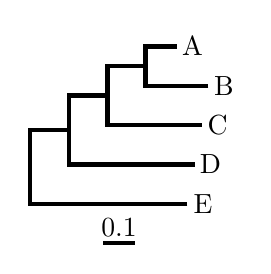
\begin{tikzpicture}[ultra thick]

\node at (-0.2, 0.0) {A};
\node at (0.2, -0.5) {B};
\draw (-0.4, 0.0) -- (-0.8, 0.0) -- (-0.8, -0.25);
\draw (0.0, -0.5) -- (-0.8, -0.5) -- (-0.8, -0.25);
\node at (0.12000000000000001, -1.0) {C};
\draw (-0.8, -0.25) -- (-1.28, -0.25) -- (-1.28, -0.625);
\draw (-0.08, -1.0) -- (-1.28, -1.0) -- (-1.28, -0.625);
\node at (0.028000000000000025, -1.5) {D};
\draw (-1.28, -0.625) -- (-1.772, -0.625) -- (-1.772, -1.0625);
\draw (-0.172, -1.5) -- (-1.772, -1.5) -- (-1.772, -1.0625);
\node at (-0.06559999999999999, -2.0) {E};
\draw (-1.772, -1.0625) -- (-2.2656, -1.0625) -- (-2.2656, -1.53125);
\draw (-0.2656, -2.0) -- (-2.2656, -2.0) -- (-2.2656, -1.53125);

\draw (-0.9328000000000001, -2.5) -- (-1.3328000000000002, -2.5);
\node at (-1.1328, -2.3) {0.1};

\end{tikzpicture}

\end{centering}

\bigskip{}

\begin{centering}

(b) phylogram

\end{centering}

\column{0.33\textwidth}

%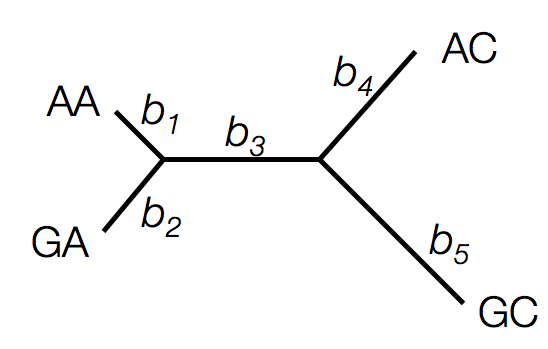
\includegraphics[width=\textwidth]{unrootedTree}

\begin{centering}


% Auto-generated from TikzTree.java
% xScale=3.0 yScale=-1.2566370614359172 offset=0.2
% scalebar=scalebar{size= 0.1 visible=true}
% options=[ultra thick]
% newick=((((A: 0.1, B: 0.2): 0.12, C: 0.3): 0.123, D: 0.4): 0.1234, E: 0.5);
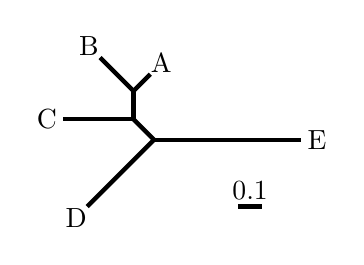
\begin{tikzpicture}[ultra thick]

\node at (-0.27757, 0.97448) {A};
\node at (-1.19681, 1.18661) {B};
\draw (-0.63112, 0.62092) -- (-0.41899, 0.83305);
\draw (-0.63112, 0.62092) -- (-1.05539, 1.04519);
\node at (-1.73112, 0.26092) {C};
\draw (-0.63112, 0.26092) -- (-0.63112, 0.62092);
\draw (-0.63112, 0.26092) -- (-1.53112, 0.26092);
\node at (-1.36015, -0.98995) {D};
\draw (-0.3702, 0) -- (-0.63112, 0.26092);
\draw (-0.3702, 0) -- (-1.21873, -0.84853);
\node at (1.7, -0) {E};
\draw (0, 0) -- (-0.3702, 0);
\draw (0, 0) -- (1.5, -0);

\draw (0.6996, -0.8485281374238571) -- (0.9996, -0.8485281374238571);
\node at (0.8496, -0.6485281374238572) {0.1};

\end{tikzpicture}

(c) unrooted tree

\end{centering}

\end{columns}

\medskip{}

\begin{columns}

\column{0.3\textwidth}

\begin{centering}

\scriptsize{((((A, B), C), D), E);}

\end{centering}

\column{0.7\textwidth}

\begin{centering}

\scriptsize{((((A:0.1, B:0.2):0.12, C:0.3):0.123, D:0.4):0.1234, E:0.5);}

\end{centering}

\end{columns}

\bigskip{}

\begin{centering}

branches (edges) and their lengths, nodes, tips (leaves)

\end{centering}

\end{frame}
